%%A Presentation by Krishna Vaidyanathan

\documentclass[aspectratio=169]{beamer}

\usepackage{hyperref}
\usepackage{color}
\usepackage{multirow}
%\usepackage[font=tiny,labelfont=bf]{caption}[numbered]

%% Smart underlining -- from cdi-macros.tex
\def\ul#1{$\underline{\smash{\hbox{#1}}}$}

%% Shortcuts

\newcommand{\tabitem}{~~\llap{\textbullet}~~}

\newcommand{\bd}{\begin{description}}
\newcommand{\ed}{\end{description}}

\mode<presentation>
{
  \usetheme{Madrid}
  \useinnertheme{circles}
  \usecolortheme{beaver}
}
\usepackage[english]{babel}

\usepackage{times}
\usepackage[T1]{fontenc}
%
\title[IceFS]{Physical Disentanglement in a Container-Based File System}
\subtitle{A Presentation for CS854}
\author[Presented by Krishna Vaidyanathan]{Lanyeu Lue,\\Yupu Zhang,\\Thanh
    Do,\\Samer Al-Kiswany,\\Andrea C. Arpaci-Dussueau,\\Remzi
    H. Arpaci-Dussueau\\\vspace{2em}Presented by Krishna Vaidyanathan}

\date{March 4, 2016}
\newcommand{\bi}{\begin{itemize}}
\newcommand{\ei}{\end{itemize}}

\newcommand{\bn}{\begin{enumerate}}
\newcommand{\en}{\end{enumerate}}

\begin{document}

\frame[plain]{\titlepage}

\begin{frame}{Table of Contents}
\tableofcontents
\end{frame}

\section{Introduction}
\begin{frame}{Introduction}
    \bi
\item Isolation is central to increased reliability and improved performance of
    modern computer systems.
\item We say, for example, that two files are \textit{entangled} if their
    blocks are allocated using the same bitmap.
\item Entanglement mainly arises because:
    \bi
\item Logically-independent file system entities are not physically independent.
    \ei
    \ei
\end{frame}

\section{Motivation}
\begin{frame}{Motivation}
    \bi
\item Entanglement can cause three main problems:
    \bn
\item Global failure
\item Slow recovery
\item Bundled performance
    \en
    \ei
\end{frame}

\begin{frame}{Global Failure}
    \begin{columns}[T]
        \begin{column}{0.5\textwidth}
        \bi
    \item Single fault leads to a global failure.
    \item Current file systems crash entire system or mark whole file system read
        -only.
    \item For example:
        \bi
    \item Btrfs crashes entire OS when invariant is violated.
    \item ext3 marks whole file-system read-only when it detects corruption in
        single inode bitmap.
        \ei
        \ei
\end{column}
\hspace{-2cm}\begin{column}{0.2\textwidth}
    \pause
    \begin{figure}\flushleft
        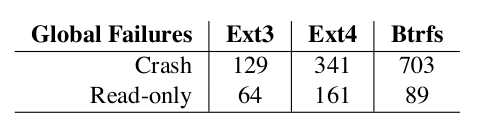
\includegraphics[scale=0.3]{./figures/table1.png}
    \end{figure}
    \pause
    \begin{figure}\flushleft
        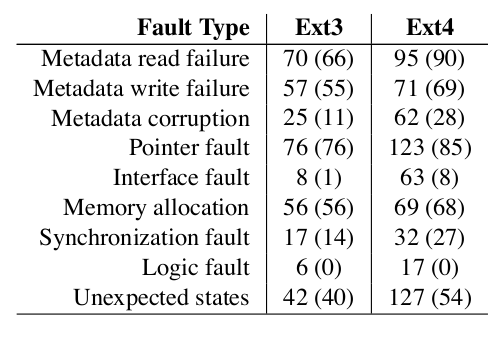
\includegraphics[scale=0.3]{./figures/table2.png}
    \end{figure}
\end{column}
\end{columns}
\end{frame}

\begin{frame}{Slow Recovery}
    \begin{columns}[T]
        \begin{column}{0.4\textwidth}
        \bi
    \item After failure, offline file-system checker scans whole file system.
    \item Checkers are pessimistic: entire file system checked, when only a small
        piece of corrupted data.
    \item Not scalable.
        \ei
    \end{column}
    \begin{column}{0.2\textwidth}
        \pause
        \begin{figure}
            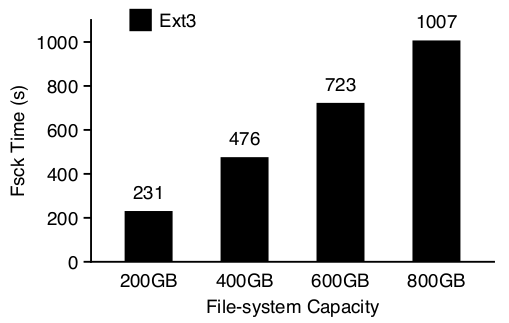
\includegraphics[scale=0.3]{./figures/fig1.png}
        \end{figure}
    \end{column}
    \end{columns}
\end{frame}

\begin{frame}{Bundled Performance}
    \begin{columns}[T]
        \begin{column}{0.4\textwidth}
            \bi
        \item File-systems, like ext3, use a journal to keep track of uncommitted changes,
            committing at periodic intervals.
        \item All updates within a short period of time are grouped together.
        \item Performance of independent processes are bundled.
            \ei
    \end{column}
    \begin{column}{0.2\textwidth}
        \pause
        \begin{figure}
            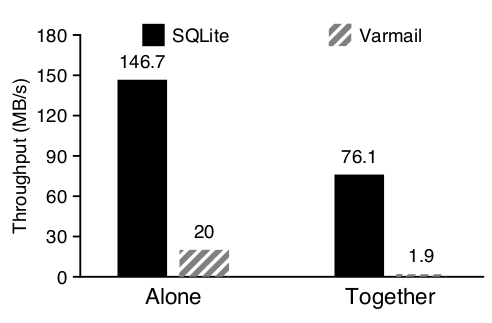
\includegraphics[scale=0.3]{./figures/fig2.png}
        \end{figure}
    \end{column}
\end{columns}
\end{frame}

\begin{frame}{Current Solutions}
    \bi
\item Namespaces: defines subset of files and directories to be made visible.
    \pause
    \bi
\item Fails to address above problems.
\item Files from different namespaces may still share metadata, system states
    etc.,
    \ei
\item Static disk partitions: Multiple file systems can be created on separate
    partitions.
    \pause
    \bi
\item Single \texttt{panic()} or \texttt{BUG\_ON()} can still crash entire OS.
\item Not flexible, and number of partitions limited.
    \ei
    \ei
\end{frame}

\begin{frame}{Usage Scenarios}
    \bi
\item Virtual Machines:
    \bi
    \pause
\item Fault isolation of paramount importance.
\item Single fault triggered by one virtual disk can cause host file system to
    become read-only.
\item Redeployment and recovery require considerable downtime.
    \ei
    \pause
\item Distributed File Systems:
    \bi
    \pause
\item Physical entanglement negatively impacts distributed file systems, especially multi-tenant
    settings.
\item Specifically, HDFS does not provide fault isolation for applications.
\item Scenario: four clients concurrently read different files, and the machine
    which stores the data blocks crashes.
    \ei
    \ei
\end{frame}

\end{document}
